\chapter{High-energy nuclear physics}
\section{Quantum Chromodynamics}
\lettrine[lines=6,findent=0.pt]{I}{n} the mid-20$^{\mathrm{th}}$ century, the realm of particle physics underwent a transformative phase, marked by the discovery of a seemingly endless variety of subatomic particles. This era witnessed the unveiling of numerous mesons and baryons, which left physicists with the necessity of developing a framework that could describe the behaviour of these particles and their interactions. This led to the development of the static quark model, which emerged in the 1960s as a groundbreaking conceptual framework to categorize the various observed particles. Developed independently by Murray Gell-Mann\cite{Gell-Mann:1964ewy} and George Zweig\cite{Zweig:1964jf, Fritzsch:1972jv}, this model postulated the existence of fundamental constituents called quarks, which, in order to reflect the experimental findings, had to be fermions (to describe baryons with spin 1/2 and 3/2) with fractional electric charge. The quark model beautifully explained the organization of hadrons in terms of three quarks ($u$, $d$, and $s$), leading to the development of a more structured and coherent classification of particles.

Despite the phenomenological success of the static quark model, it had two problems: it introduced particles with fractional charge, which had never been observed before, and, most importantly, it gave rise to a violation of the Fermi-Dirac statistics. The $\Delta^{++}$, $\Delta^{-}$, and $\Omega^{-}$ baryons, in fact, have symmetric orbital, spin and flavour wavefunctions, which defied the Pauli exclusion principle that should have implied antisymmetric wavefunctions for these particles.

To resolve these inconsistencies, a new degree of freedom, the \emph{colour}, was introduced. Hadrons wavefunctions were assumed to be totally antisymmetric in colour quantum numbers, effectively implementing the Pauli exclusion principle.

The simplest model of colour would be to assign quarks to the fundamental representation of a global $SU(3)$ symmetry. Each quark now carries a colour index: $q_i$, where $i = 1, 2, 3$, and transforms under the fundamental ($3$) representation of $SU(3)$, while antiquarks,  $\bar{q}_i$, transform in the $\bar{3}$ representation. Introducing the totally antisymmetric tensor $\varepsilon^{ijk}$, possible compositions of quarks that give rise to colour singlets are 
\begin{equation*}
    \bar{q}^iq_i,\qquad \varepsilon^{ijk}q_iq_jq_k,\qquad \varepsilon^{ijk}\bar{q_i}\bar{q_j}\bar{q_k},
\end{equation*}
which are the quarks compositions of mesons, baryons, and antibaryons, respectively. 

One of the tests supporting the existence of colour and fractional electric charge came in the form of the ratio R, of the $\mathrm{e}^+ \mathrm{e}^-$ total hadronic cross-section to the cross-section of a pair of muons produced from the same annihilation process. The virtual photon emitted in the annihilation can produce all electrically charged pairs of particles and antiparticles, as shown in Fig.~\ref{fig:ee_to_ff_diagram}.
\begin{figure}[h]
    \centering
        \feynmandiagram [horizontal=a to b] {
          i1 [particle=\(e^{-}\)] -- [fermion] a -- [fermion] i2 [particle=\(e^{+}\)],
          a -- [photon, edge label=\(\gamma^*\)] b,
          f1 [particle=\(\bar{f}\)] -- [fermion] b -- [fermion] f2 [particle=\(f\)],
        };
\caption{$\mathrm{e}^+ \mathrm{e}^-$ annihilation to a pair of fermions}
    \label{fig:ee_to_ff_diagram}
\end{figure}

The ratio R is given by:
\begin{equation*}
    R = \frac{\sigma(e^+e^- \rightarrow hadrons)}{\sigma(e^+e^- \rightarrow \mu^+\mu^-)} = N_c \sum_f Q_f^2\ ,
\end{equation*}
where $N_c$ represents the number of existing colours and $Q_f$ is the electric charge of the quark flavour $f$. Notably, this ratio is dependent on the energy of the center-of-mass system and encompasses all possible quark flavors that can be produced by the virtual photon at that specific energy level. The experimental data for $R$ (shown in Fig.~\ref{fig:R_vs_s}) exhibited a remarkable agreement with the predictions of the three-color model, thereby providing compelling evidence for the existence of color and fractional electric charge of quarks.

The final step that propelled the development of Quantum Chromodynamics (QCD) as a comprehensive theory of the strong force was the insight into the mechanism that ensured all hadron wavefunctions to be color singlets. This emerged from the discovery of asymptotic freedom, a phenomenon observed in deep-inelastic scattering experiments. Non-Abelian gauge theories, often referred to as Yang-Mills theories, were identified as having this unique characteristic. This realization led to the formulation of QCD by elevating the global color $SU(3)$ symmetry to a local one, allowing the 8 quanta of the $SU(3)$ gauge field, called \emph{gluons}, to mediate the strong force, successfully describing the confinement and behavior of quarks and gluons within hadrons.

\begin{figure}[p]
    \centering
    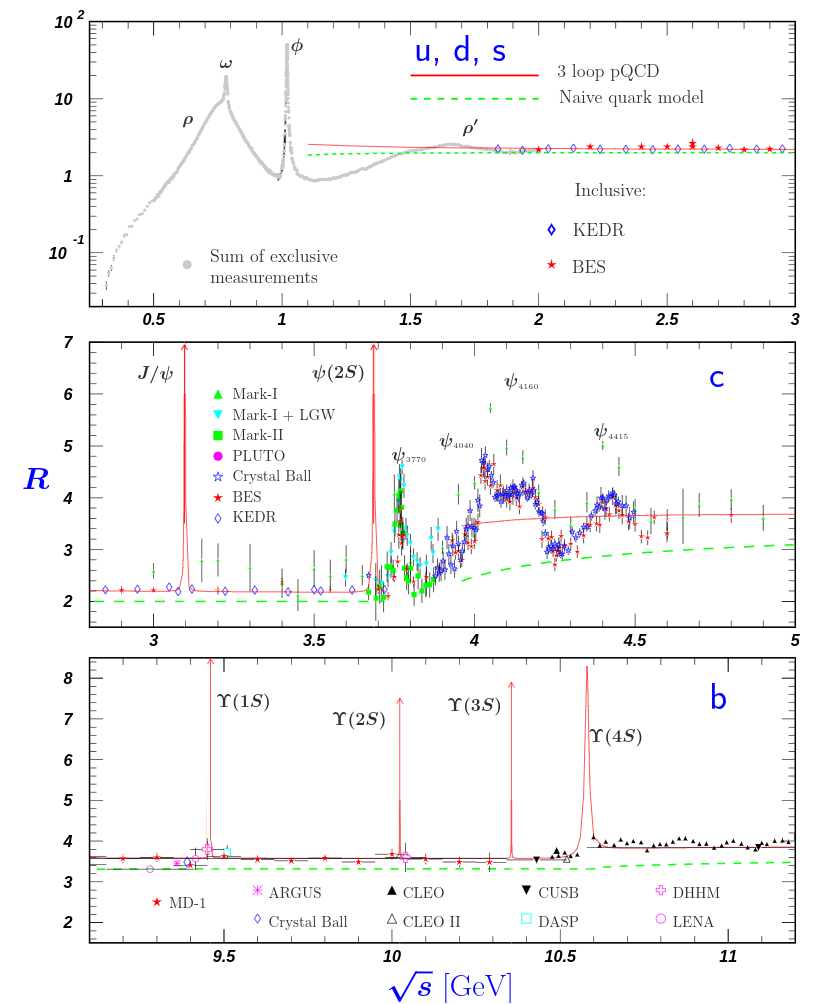
\includegraphics[width=\linewidth]{Figures/Chapter 1/rpp2022-R_udscb.pdf}
    \caption{$R$ as a function of $\sqrt{s}$ in the light-flavor, charm, and beauty threshold regions taken from \cite{pdg}. The green curve is a naive quark-parton model prediction, while the red one is a 3-loops perturbative QCD prediction. Breit-Wigner parameterizations of $J/\psi$, $\psi$(2S), and $\Upsilon$(nS), n = 1,2,3,4 are also shown}
    \label{fig:R_vs_s}
\end{figure}

The QCD Lagrangian density can be written as:
\begin{equation}\label{eq:Lqcd}
    \mathcal{L}_{QCD}=-\frac{1}{4} F^a_{\mu\nu}F_a^{\mu\nu} + \sum_f \bar{q}_f^i (i\gamma^\mu(\mathcal{D}_\mu)_{ij}-m_f\delta_{ij})q_f^j\ ,
\end{equation}
where $F^a_{\mu\nu}$ is the field strength tensor defined in terms of the gluon field $A^a_\mu$ and the $SU(3)$ structure constant $f^{abc}$:
\begin{equation} \label{eq:F}
    F^a_{\mu\nu} = \partial_\mu A^a_\nu - \partial_\nu A^a_\mu + g_s f^{abc}A^b_\mu A^c_\nu 
\end{equation}
and $(\mathcal{D}_\mu)_{ij}$ is the covariant derivative:
\begin{equation*}
    (\mathcal{D}_\mu)_{ij} = \partial_\mu \delta_{ij} - ig_s(t^a)_{ij}A_\mu^a\ ,
\end{equation*}
with $t^a$ being one of the generators of the $SU(3)$ representation.

The last term in Eq.~\ref{eq:F} is peculiar to non-Abelian theories, and gives rise to triplet and quartic gluon self-interactions illustrated in Fig.~\ref{fig:Feynman-gluons}. $g_s$ is a coupling parameter related to the coupling constant \als, which determines the strength of the interaction between the coloured particles.

\begin{figure}[htb]
    \centering
    \begin{tikzpicture}
      \begin{feynman}
        \vertex (a) {a};
        \vertex [right=of a] (b);
        \vertex[above right= of b] (c) {b};
        \vertex[below right= of b] (d) {c};
        \diagram* {
          (a) -- [gluon] (b),
          (b) -- [gluon] (c),
          (b) -- [gluon] (d),
        };
      \end{feynman}
    \end{tikzpicture} \qquad
    \begin{tikzpicture}
      \begin{feynman}
        \vertex (a);
        \vertex[above left=of a] (b) {a};
        \vertex[above right= of a] (c) {b};
        \vertex[below right= of a] (d) {c};
        \vertex[below left= of a] (e) {d};
        \diagram* {
          (a) -- [gluon] (b),
          (a) -- [gluon] (c),
          (a) -- [gluon] (d),
          (a) -- [gluon] (e),
        };
      \end{feynman}
    \end{tikzpicture}
    \caption{Feynman diagrams for gluons self-interactions}
    \label{fig:Feynman-gluons}
\end{figure}

The second term of Eq.~\ref{eq:Lqcd} describes the interactions between quarks and gluons, sketched in Fig.~\ref{fig:Feynman_q_g}, and contains the mass term for the fermions. It is noteworthy to observe that the interaction between quarks and gluons is diagonal in flavor, meaning that the strong interaction conserves the flavor of quarks. In contrast, colour mixing is allowed within the framework of QCD.

\begin{figure}[htb]
    \centering
    \begin{tikzpicture}
      \begin{feynman}
        \vertex (a);
        \vertex [below=0.1em of a] {$t^a_{ij}$};
        \vertex[left=of a] (b) {$q_i$};
        \vertex[right= of a] (c) {$q_j$};
        \vertex[above right= of a] (d) {a};
        \diagram* {
          (b) -- [fermion] (a),
          (a) -- [fermion] (c),
          (a) -- [gluon] (d),
        };
      \end{feynman}
    \end{tikzpicture}
    \caption{Feynman diagram for quark-gluon interaction}
    \label{fig:Feynman_q_g}
\end{figure}

\subsection{Running coupling constant}
If one considers a dimensionless physical observable, denoted in the following as $R$, which solely depends on a single energy scale, $Q$, one might naturally expect that $R$ would maintain a constant value, independent of the specific energy scale chosen. However, this does not hold true when loop diagrams are studied: the necessity of renormalisation introduces a new energy scale denoted as $\mu$. This scale, known as the renormalisation scale, is the point at which the subtraction of the ultraviolet divergences is carried out. Critically, $\mu$ is an arbitrary parameter and, as such, is non-physical. Consequently, $R$ becomes dependent on the ratio $Q^2/\mu^2$ and the renormalised coupling $\alpha_s = g_s^2/4\pi$: $R = R\left(\frac{Q^2}{\mu^2},\als\right)$. The $\mu$ independence of $R$ (which is an essential requirement given $\mu$'s arbitrariness) can be expressed as:
\begin{equation}\label{eq:RGE}
    \mu^2 \frac{\de R\left(\frac{Q^2}{\mu^2},\alpha_s\right)}{\de \mu^2} = \mu^2 \left[\frac{\partial}{\partial\mu^2}+\frac{\partial \alpha_s}{\partial\mu^2}\frac{\partial}{\partial\alpha_s}\right]R\left(\frac{Q^2}{\mu^2},\alpha_s\right) = 0\ , 
\end{equation}
a fundamental equation known as the renormalisation group equation. This equation is exactly true in the case of a prediction that considers all perturbative orders. If one limits the expansion at a fixed order $\alpha_s^N$, then a dependence of $R$ from $\mu$ is observed at the $\als^{N+1}$ order.\\ Solving Eq.~\ref{eq:RGE} requires the introduction of the concept of the running coupling $\alpha_s(Q^2)$, which evolves as a function of $Q$. By introducing
\begin{equation*}
    t\equiv \mathrm{log}(Q^2/\mu^2), \qquad \beta(\als)\equiv \mu^2 \frac{\de\als}{\mathrm{\mu^2}}\quad ,
\end{equation*}
Eq.~\ref{eq:RGE} can be written as
\begin{equation*}
    \left(-\frac{\partial}{\partial t} + \beta(\als)\frac{\partial}{\partial \als}\right) R(e^t,\als) = 0
\end{equation*}
This first-order partial differential equation can be solved by defining a new function: the running coupling $\als(Q^2)$
\begin{equation}\label{eq:t_integral}
    t = \mathrm{log}(Q^2/\mu^2) \equiv \int_{\als}^{\als(Q^2)} \frac{\de x}{\beta(x)} , \quad \mathrm{with}~\als=\als(\mu^2)\quad .
\end{equation}
By differentiating Eq.~\ref{eq:t_integral} with respect to $t$ and \als, one gets:
\begin{equation}\label{eq:beta_def}
    \beta(\als(Q^2)) = \frac{\partial\als(Q^2)}{\partial t}, \quad \frac{\de\als(Q^2)}{\de\als} = \frac{\beta(\als (Q^2))}{\beta(\als)}\quad .
\end{equation}
It results from this last set of equations that $R(1,\als(Q^2))$ satisfies Eq.~\ref{eq:RGE}; hence, the running coupling constant has absorbed the $\mu$ scale dependence of $R$. As a consequence, the knowledge of $R(1,\als)$, which can be evaluated in fixed-order perturbation theory, allows to know the dependence of $R$ from $Q^2$, the physical scale at which the coupling is gauged, by simply substituting $\als \rightarrow \als(Q^2)$. 

\subsubsection{The \ensuremath{\beta} function}
The running of the coupling constant is determined by the $\beta(\als)$ function, which is evaluated from loop corrections to the bare vertices of the theory. As of the time of the writing of this Thesis, the $\beta$ function has been evaluated up to 5 loops\cite{Herzog:2017ohr}. In Fig.~\ref{fig:beta_loops}, the 1-loop Feynman diagrams contributing to the $\beta$ function evaluation are reported.

\begin{figure}[htb]
    \centering
    \begin{tikzpicture}
      \begin{feynman}
        \vertex (a);
        \vertex [right=1cm of a] (b);
        \vertex[right=1cm of b] (c);
        \vertex[right=1cm of c] (d);
        \diagram* {
            (a) -- [gluon] (b)
            -- [fermion, half left, looseness=1.5] (c)
            -- [fermion, half left, looseness=1.5] (b),
            (c) -- [gluon] (d),
        };
      \end{feynman}
    \end{tikzpicture}\quad
    \begin{tikzpicture}
      \begin{feynman}
        \vertex (a);
        \vertex [right=1cm of a] (b);
        \vertex[right=1cm of b] (c);
        \vertex[right=1cm of c] (d);
        \diagram* {
            (a) -- [gluon] (b)
            -- [gluon, half left, looseness=1.5] (c)
            -- [gluon, half left, looseness=1.5] (b),
            (c) -- [gluon] (d),
        };
      \end{feynman}
    \end{tikzpicture}\quad
    \begin{tikzpicture}
      \begin{feynman}
        \vertex (a);
        \vertex [right=of a] (b);
        \vertex[above=1cm of b] (c);
        \vertex[right=of b] (d);
        \diagram* {
            (a) -- [gluon] (b)
            -- [gluon, half left, in=90, looseness=2] (c)
            -- [gluon, half left, in=90, looseness=2] (b),
            (b) -- [gluon] (d),
        };
      \end{feynman}
    \end{tikzpicture}\quad

    \vspace{0.6cm}
    \begin{tikzpicture}
      \begin{feynman}
        \vertex (a);
        \vertex [right=1cm of a] (b);
        \vertex[right=1cm of b] (c);
        \vertex[right=1cm of c] (d);
        \diagram* {
            (a) -- [gluon] (b)
            -- [ghost, half left, looseness=1.5] (c)
            -- [ghost, half left, looseness=1.5] (b),
            (c) -- [gluon] (d),
        };
      \end{feynman}
    \end{tikzpicture}\quad
    \begin{tikzpicture}
      \begin{feynman}
        \vertex (a);
        \vertex [right=1cm of a] (b);
        \vertex[right=1cm of b] (c);
        \vertex[right=1cm of c] (d);
        \vertex[below=0.31cm of c] (f) {$ $};
        \diagram* {
            (a) -- [fermion] (b) -- [fermion] (c) -- [fermion] (d),
            (b) -- [gluon, half left, looseness=1.5] (c)
            
        };
      \end{feynman}
    \end{tikzpicture}\quad
    
    \vspace{0.5cm}
    \begin{tikzpicture}
      \begin{feynman}
        \vertex (a);
        \vertex [right=1cm of a] (b);
        \vertex[above right=1cm of b] (c);
        \vertex[right=1cm of c] (d);
        \vertex[below right=1cm of b] (e);
        \vertex[right=1cm of e] (f);
        \diagram* {
            (a) -- [gluon] (b) -- [fermion] (c) -- [fermion] (d),
            (b) -- [fermion] (e) -- [fermion] (f),
            (c) -- [gluon] (e)
        };
      \end{feynman}
    \end{tikzpicture}\quad
    \begin{tikzpicture}
      \begin{feynman}
        \vertex (a);
        \vertex [right=1cm of a] (b);
        \vertex[above right=1cm of b] (c);
        \vertex[right=1cm of c] (d);
        \vertex[below right=1cm of b] (e);
        \vertex[right=1cm of e] (f);
        \diagram* {
            (a) -- [gluon] (b) -- [gluon] (c),
            (b) -- [gluon] (e),
            (f) -- [fermion] (e) -- [fermion] (c) -- [fermion] (d)
        };
      \end{feynman}
    \end{tikzpicture}\quad
    \caption{1-loop Feynman diagrams contributing to the $\beta$ function evaluation}
    \label{fig:beta_loops}
\end{figure}

By limiting the calculations at the first order in the perturbative expansion, one gets:
\begin{equation}\label{eq:beta0}
    \beta(\als) = -\als^2 \frac{11 \mathrm{N_c} - 2 \mathrm{N_f}}{12\pi} + \mathcal{O}(\als^3) \equiv -\als^2 \beta_0 + \mathcal{O}(\als^3)\quad ,
\end{equation}
where $\mathrm{N_c}$ is the number of colours (3), while $\mathrm{N_f}$ is the number of quark flavours which can be considered massless at the physical scale $Q^2$ at which the coupling is being measured.
From Eqs.~\ref{eq:beta0} and \ref{eq:beta_def}, one can extract the $Q^2$ dependency of the running coupling constant:
\begin{equation}\label{eq:alpha_s_running}
    \alpha_s(Q^2) = \frac{\alpha_s(\mu^2)}{1+\alpha_s(\mu^2)\beta_0 \mathrm{log}(Q^2/\mu^2)}\ ,
\end{equation}
Notably, since $\beta_0$ is positive in a 6 quark-flavours framework, the strong coupling constant exhibits a monotonic decreasing trend as a function of $Q^2$. This behaviour differs from the one of the electromagnetic coupling constant, which increases with the energy scale due to the screening effect of vacuum polarisation. For QCD, the running of the coupling constant is a direct consequence of the non-Abelian nature of the theory, allowing for gluon self-interactions, which give rise to an anti-screening effect. The idea is that the emission of virtual gluons by static colour sources causes their colour charges to 'leak out' into the surrounding vacuum. Since the interaction between distributions of charges is weaker than the one between point-like charges when the distributions overlap, the effective coupling constant decreases at short distances. This behaviour is known as asymptotic freedom, a key feature of QCD that allows for the perturbative expansion of the theory at high energy scales, where the strong coupling constant is small. At the same time, the running of the coupling constant implies that the theory is non-perturbative at low energy scales, and phenomenological models are required to describe the strong interaction in this regime. 

Instead of using the renormalisation scale $\mu$ as a free parameter, one can use the running coupling constant to define a physical scale, $\Lambda_{QCD}$, which is the energy scale at which the coupling constant would diverge, if extrapolated outside the perturbative regime. Using Eq.~\ref{eq:alpha_s_running}, one can write:
\begin{equation*}
    \alpha_s(\Lambda_{QCD}) = \frac{1}{\beta_0 \mathrm{log}(Q^2/\Lambda_{QCD}^2)}\quad .
\end{equation*}
The value of $\Lambda_{QCD}$ is determined by the specific definition being used. However, to obtain the value of the coupling constant measured at $Q^2 = M_Z^2$, an approximate value of $\Lambda_{QCD}$ of around 200 MeV can be used.

Measurements of the running of the coupling constant at different values of $Q$ are illustrated in Fig.~\ref{fig:alpha_s_running} and compared to the theoretical prediction at 5 loops. The agreement between the experimental data and the theoretical prediction is remarkable, confirming the validity of the QCD framework at high energy scales.


\begin{figure}[htb]
    \centering
    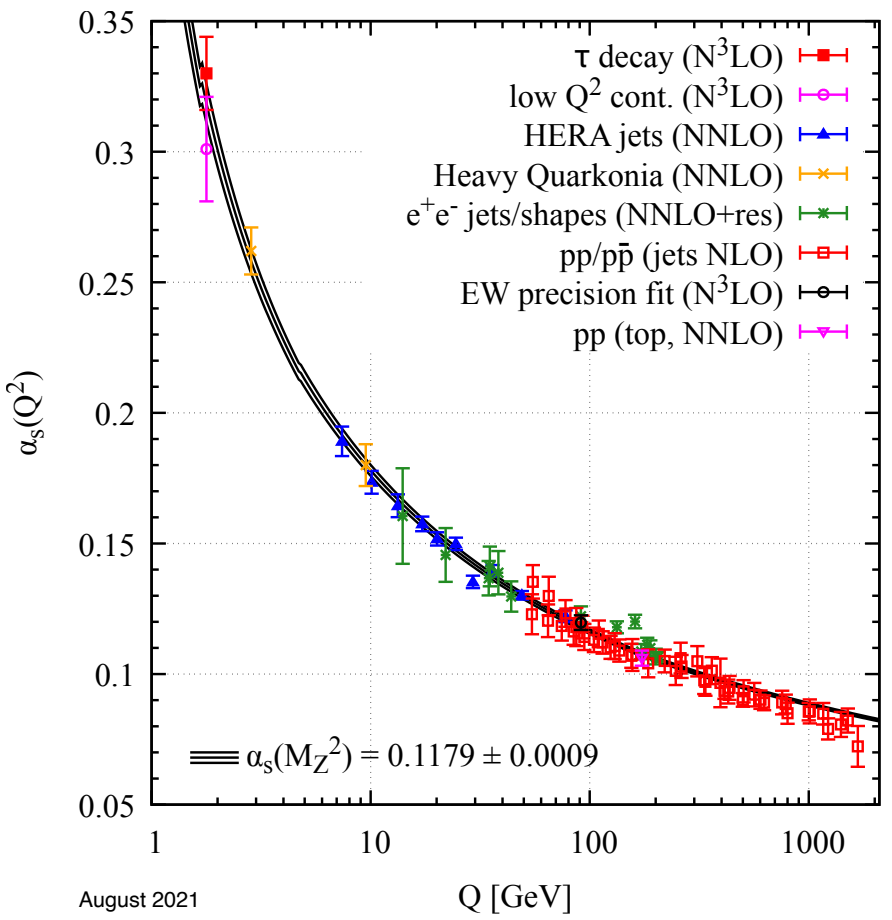
\includegraphics[width=0.7\linewidth]{Figures/Chapter 1/Alpha_s_running.png}
    \caption{Summary of measurements of \als as a function of the energy scale $Q$, compared to the running of the coupling computed at five loops, taking as an input the current PDG average, $\als(M_Z^2) = 0.1180 \pm 0.0009$ \gevcc. Taken from \cite{pdg}}
    \label{fig:alpha_s_running}
\end{figure}

\section{Confinement}
The concept of confinement is one of the most intriguing aspects of QCD. It is the phenomenon by which quarks and gluons are never observed as free particles, but are always confined within colour-neutral hadrons. The confinement of quarks and gluons is a direct consequence of the non-Abelian nature of the theory, which, as described in the previous Section, is characterised by an increase of the strong coupling constant at low energy scales. The confinement of quarks and gluons is a non-perturbative effect, and despite extensive research, a comprehensive theoretical description of confinement in QCD remains elusive. Phenomenological models like the MIT bag model have been proposed, but a full comprehension of confinement is still lacking. Lattice QCD simulations are the most successful approach to study the non-perturbative regime of the theory, and they have provided a wealth of information on the properties of hadrons and the strong interaction at low energy scales.

\subsection{MIT bag model}
The MIT bag model~\cite{Johnson:1975zp} is a phenomenological model of confinement, which describes hadrons as bound states of quarks and gluons confined within a finite volume, called the bag. The model was developed in the 1970s by A. Chodos, R. L. Jaffe, K. Johnson, C. B. Thorn, and V. F. Weisskopf, and it has been widely used to study the properties of hadrons and the strong interaction. In the MIT bag model, N non-interacting massless fermions are confined within a spherical cavity of radius $R$, which is the bag radius. The confinement arises from a balance between pressure due to the kinetic energy of the fermions inside the bag and an ad hoc external pressure, which is introduced to confine the fermions within the bag. The fermions are described by the Dirac equation for massless fermions:

\begin{equation*}
    i\gamma^\mu\partial_\mu\psi = 0\quad ,
\end{equation*}
where $\psi$ is the fermion field, and $\gamma^\mu$ are the Dirac matrices. The solution to the Dirac equation is given in terms of the spherical Bessel functions of the zeroth and first order, $j_0(p_0r)$ and $j_1(p_0r)$, where $p_0$ is the energy of the fermion:

\begin{equation*}
    \psi = \mathcal{N} e^{-ip_0t} \begin{pmatrix} j_0(p_0r)\chi^+ \\ \vec{\sigma}\cdot\hat{r}j_1(p_0r)\chi^-\end{pmatrix}\quad ,
\end{equation*}
where $\chi^+$ and $\chi^-$ are the two components of the fermion four dimentional spinor $\psi$, and $\vec{\sigma}$ are the Pauli matrices. The colour flux at a point $r$ inside the bag is given by:

\begin{equation*}
    j_{ab}^\mu(r) = \bar{\psi_a}(r)\gamma^\mu\psi_b(r)\quad ,
\end{equation*}
where $a$ and $b$ are the colour indices of the fermions. If the quantum numbers are not to be lost through the surface of the bag, which is the definition of confinement, then:

\begin{equation*}
  n_\mu j_{ab}^\mu(r) = \bar{\psi_a}(r)\gamma\cdot n \psi_b(r) = 0\quad 
\end{equation*}
on the surface, where $n_\mu$ is a unit space-like vector perpendicular to the surface. Using the gamma properties, $(i\gamma\cdot n)^2 = 1$, so that by assuming that $i\gamma\cdot n = + 1$, the boundary condition on the surface of the bag is given by:

\begin{equation*}
    \bar{\psi}(R)\psi(R) = 0\quad ,
\end{equation*}
leading to the solution of the Dirac equation in the bag:

\begin{equation*}
    \left[j_0\left(p_0R\right)\right]^2 - \left[j_1\left(p_0R\right)\right]^2 = 0\quad ,
\end{equation*}
with solution $p_0R = 2.04$. The total energy inside the bag is given by:

\begin{equation*}
    E = \frac{2.04 N}{R}(\hbar c) + \frac{4\pi}{3}R^3B\quad ,
\end{equation*}
where the first term is the kinetic energy of the fermions, and the second term is the energy due to the presence of an external pressure $B$ which keeps the fermions confined in the bag. The bag pressure is a phenomenological parameter of the model, and it is introduced to confine the fermions within the bag. It can be extracted by minimising the energy of the system with respect to the bag radius $R$, which yields $B=234$ MeV/fm$^3$ for a baryon with $R=0.8$ fm.

\subsection{Lattice QCD}
Lattice QCD is a numerical technique used to study the non-perturbative regime of QCD. The method is based on the discretisation of space-time on a four-dimensional lattice, and the evaluation of the path integral of the theory using Monte Carlo methods, i.e. by sampling possible configurations of the quark and gluon fields according to the probability distribution given by the QCD Lagrangian. The lattice spacing is a parameter of the method, and allows one to avoid the ultraviolet divergences of the theory, which are typical in perturbative QCD, by introducing a cutoff on the momenta of the quark and gluon fields. 
\begin{figure}[htb]
  \centering
  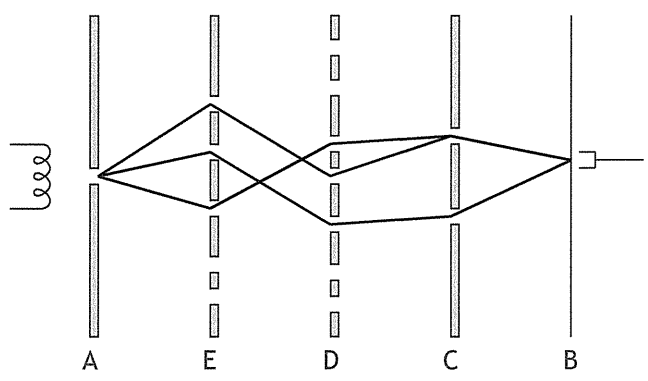
\includegraphics[width=0.7\linewidth]{Figures/Chapter 1/PathIntegrals.png}
  \caption{Feynman introduction to path integrals. Here, a particle emitted from a source at $x_a$ is detected at $x_b$. A finite number of screens, each with a finite number of holes, is placed between the source and the detector. The probability amplitude for the particle to hit the detector is given by the sum of the probabilities of moving from the source to the detector through all possible paths. By adding an infinite amount of screens with an infinite number of holes, and by also considering the time at which the particle passes through each screen, the sum becomes an integral over all possible paths, called a \emph{path integral}.}
  \label{fig:PathIntegrals}
\end{figure}

The Lattice QCD simulations are based on the path integral formalism of quantum field theory~\cite{RevModPhys.20.367}, developed by R. Feynman in the 1940s. The path integral provides a natural extension to quantum mechanics of the least action principle of classical mechanics, and it allows one to calculate the probability amplitude of a particle to move from one point to another in space-time, considering the evolution of the system over all possible paths. The transition amplitude from the state $(x_a,t_a)$ to the state $(x_b,t_b)$ is given by:
\begin{equation}\label{eq:ampl_prob}
  A \left[(x_a,t_a) \rightarrow (x_b,t_b) \right] = \braket{x_b,t_b | e^{-iH(t_b-t_a)} | x_a,t_a} = \sum_\mathrm{paths} e^{iS[x(t)]}\quad , 
\end{equation}
where $H$ is the Hamiltonian of the system, $S[x(t)]$ is the action of the system for a given path $x(t)$, and the sum is over all possible paths from $(x_a,t_a)$ to $(x_b,t_b)$. By taking the continuum limit on space-time, we obtain an integration over all the possible space-time paths of the system:
\begin{equation}\label{eq:path_integral}
  \sum_\mathrm{paths} e^{iS[x(t)]} \rightarrow \int_{x_a}^{x_b} \left[\mathcal{D}x(t)\right] e^{iS[x(t)]}\quad ,
\end{equation}
where the right-hand side term is a functional integral over all possible paths. It is interesting to note that by combining Eqs.~\ref{eq:ampl_prob} and \ref{eq:path_integral}, one gets a quantity resembling the partition function of a statistical system:
\begin{equation*}
  \mathcal{Z} = \sum_{x_a} \braket{x_a,t_a | e^{\beta H} | x_a,t_a}\quad .
\end{equation*}
It is possible to express the partition function in terms of a path integral by applying a Wick rotation to the time variable, $t \rightarrow -i\tau$, with $\tau_a~=~0~\leq~\tau~\leq~\tau_b~=~\beta$ and considering the Euclidean action in place of the Minkowskian one, $S_E~=~iS$. Furthermore, since the state at $\tau_a$ is the same as the one at $\tau_b$ in the partition function definition, a periodic boundary condition is imposed: $x(\tau_a) = x(\tau_b)$. With these considerations, the partition function can be expressed as:
\begin{equation*}
  \mathcal{Z} = \int \left[\mathcal{D}x(\tau)\right] e^{-S_E[x(\tau)]}\quad .
\end{equation*}
This formalism, which was here developed for a single particle, can be extended to a quantum field theory, and in particular to QCD.

Lattice QCD simulations are computationally intensive, and they require large supercomputers to perform the calculations. To limit the computational costs, calculations are often performed at larger up and down quark masses than in nature, drastically reducing the number of virtual quark-antiquark loops that have to be taken into account. Because of the employed Monte Carlo approach, only a finite number of configurations can be considered, leading to statistical uncertainties in the lattice QCD results. In order to obtain physical results, several limits have to be taken: i. the continuum limit, i.e. the extrapolation of the lattice spacing to zero, ii. the infinite-volume limit, i.e. the extrapolation of the lattice size to infinity, and iii. the physical quark-mass limit, i.e. the extrapolation to physical quark masses. Many present-day lattice calculations are already performed directly at, or very close to, the physical values of the quark masses, so that the latter extrapolation becomes less of an issue. 

The results of the lattice QCD simulations are in good agreement with the experimental data as shown in Fig.~\ref{fig:LQCD_hadron_mass} for the spectrum of hadrons obtained from lattice QCD simulations, taken from~\cite{BMW:2008jgk}, compared to the experimental data.
\begin{figure}[t!]
  \centering
  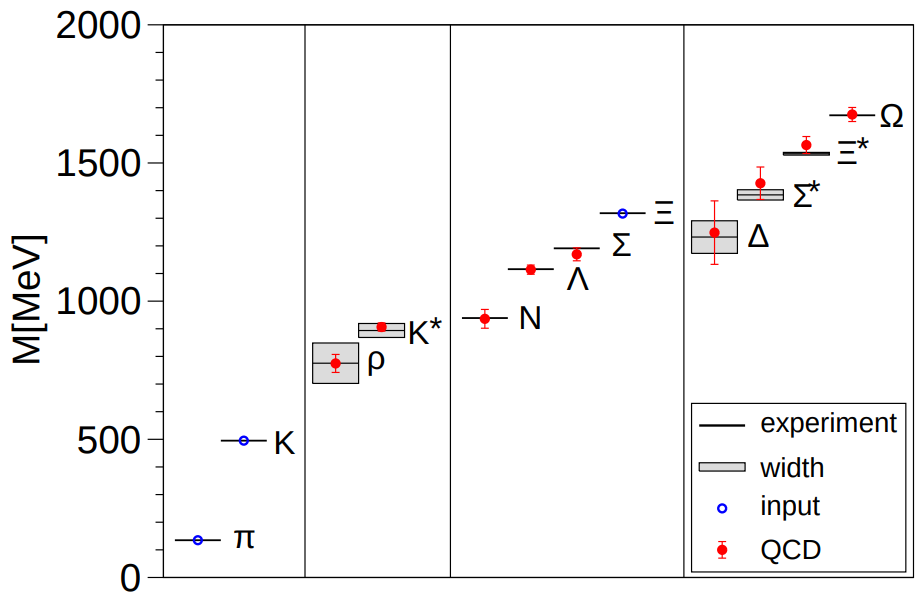
\includegraphics[width=0.7\linewidth]{Figures/Chapter 1/LQCD_hadron_mass.png}
  \caption{The light hadron spectrum of QCD. Horizontal lines and bands are the experimental values with their decay widths. Lattice QCD results~\cite{BMW:2008jgk} are shown by solid circles. Vertical error bars represent the combined statistical and systematic error estimates. $\pi$, K and $\Xi$ have no error bars, because they are used to set the light quark mass, the strange quark mass, and the overall scale, respectively.}
  \label{fig:LQCD_hadron_mass}
\end{figure}

\section{Quark Gluon Plasma}
The concept of deconfinement refers to the transition from a confined state to a state where quarks and gluons are no longer confined within hadrons, but are free to move in a larger volume. As modelled by the MIT bag model, non-perturbative QCD effects can be described in terms of an external pressure, which confines quarks and gluons within a finite volume. If the external pressure is overcome by the pressure due to the kinetic energy of the quarks and gluons, then the hadrons constituents are no longer confined, and a transition to a state called Quark-Gluon Plasma (QGP) occurs. Lattice QCD calculations are used to understand the properties of the QGP, and they predict that a strongly interacting system with zero net baryon density evolves smoothly from a confined (hadronic) towards a deconfined (quarks and gluons) state when its temperature is increased up to $\sim155$ MeV ($1.8\times 10^{12}$ K)~\cite{HotQCD:2014kol, Borsanyi:2013bia}, reaching energy densities of $\sim 1$~GeV/fm$^3$.

\begin{figure}
  \centering
  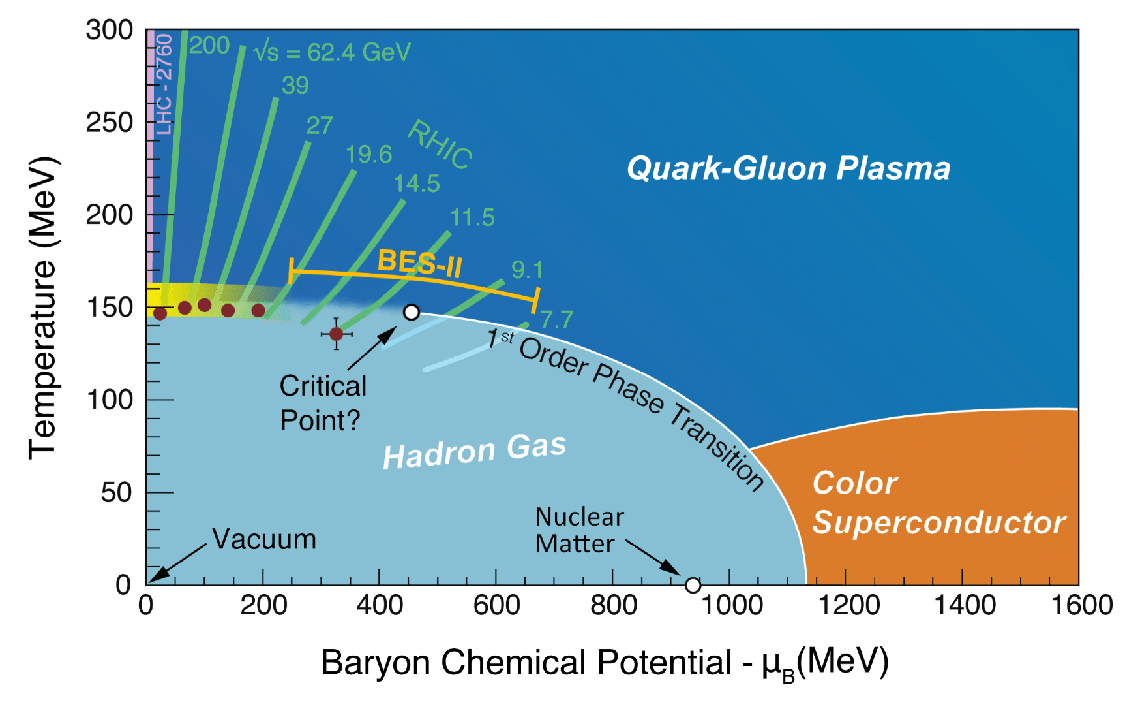
\includegraphics[width=0.7\linewidth]{Figures/Chapter 1/QCD-diagram.jpg}
  \caption{QCD phase diagram in the temperature-baryon chemical potential plane. Taken from~\cite{QCD_diagram}.}
  \label{fig:PhaseDiagram}
\end{figure}

It is believed that the universe underwent a phase of deconfinement in the early stages of its evolution, a few microseconds after the Big Bang. Direct observation of the primordial QGP (i.e. that created just after the Big Bang) would provide a wealth of information on the early universe; however, the universe experienced a phase in which electrons were not bound to nuclei (electromagnetic plasma), making it opaque to electromagnetic radiation, and denying us the possibility of directly observing the primordial QGP. Once the universe cooled enough (3000~K) to allow electrons to bind to nuclei, the electromagnetic radiation decoupled with a black body spectrum of around 3000 K. Since then, as the universe expanded, this electromagnetic radiation has redshifted to a temperature of around 2.7~K, and is denoted as the Cosmic Microwave Background (CBM). The CMB is the oldest light in the universe and provides a snapshot of the universe when it was 300'000 years old, long after the QGP had already cooled down. Hence, the only way to study the QGP is by recreating it in laboratories, through the collision of heavy ions at high energies. In the past decades, several experiments~\cite{ALICE:2022wpn, NA38:2000wlp, NA50:1997hlx, Nouicer:2009fy} have been carried out to study the properties of this state of matter, and the results have provided valuable insights into the properties of the strongly-interacting matter.

\subsection{Heavy-ion collisions}
\begin{figure}[t]
  \centering
  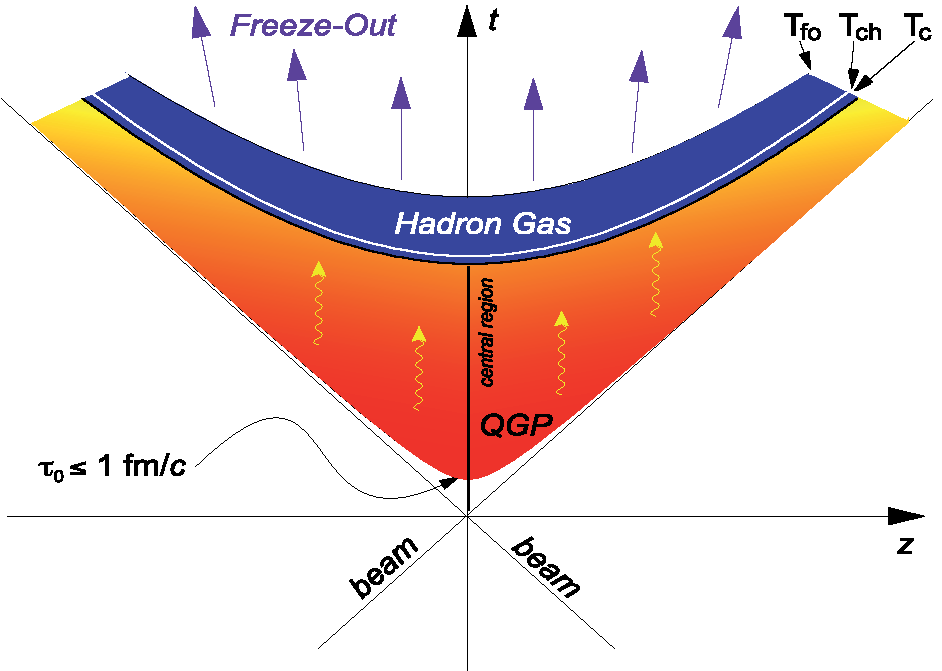
\includegraphics[width=0.7\linewidth]{Figures/Chapter 1/Bild_18.pdf}
  \caption{Space-time evolution of a heavy-ion collision. Taken from~\cite{Stock:2008ru}.}
  \label{fig:HeavyIonCollisions}
\end{figure}
Heavy-ion collisions are the most suitable environment to study the properties of the QGP. In these collisions, two heavy ions, such as lead or gold nuclei, are accelerated to ultra-relativistic energies and made to collide head-on. Given the large amount of energy deposited in the collision, the system reaches high energy densities of around 16 GeV/fm$^3$ after 1 fm/$c$~\cite{Loizides:2011ys}, which allows for the production of the QGP. As nuclei are objects made of many nucleons (i.e. protons and neutrons), the interaction volume (called \emph{fireball}) is larger and longer-lived than in proton-proton collisions, allowing to use thermodynamics and fluidodynamics to describe the system. 

It is possible to distinguish between two different collision regimes. When the centre-of-mass energy per nucleon pair (\snn) is below a few GeV, the nucleons are stopped in the collision as they lose energy and momentum. Due to conserved currents, the quantum numbers of the initial state are preserved, so that, for example, the net baryon production (i.e. the difference between the number of baryons and antibaryons) is positive. This regime is called \emph{stopping regime}. When the \snn increases, the initial state baryon number is carried away by the receding nucleons, and the net baryon number in the fireball is zero. This regime is denoted as \emph{Bjorken regime}, or \emph{transparency regime}. 

The collision of two nuclei is a rather complex process, with a space-time evolution that can be divided into several stages, as depicted in Fig.~\ref{fig:HeavyIonCollisions}. They can be studied by measuring different final-state observables that are correlated to such stages. One of the first descriptions of the fireball evolution was given by Bjorken~\cite{Bjorken:1982qr}, who proposed a simple model to describe the expansion of the system in the longitudinal direction. In this model, it is assumed that there exists a central-plateau structure in the inclusive particle productions as a function of the rapidity variable, which is defined as 
\begin{equation*}
    y = \frac{1}{2}\mathrm{log}\left(\frac{E+p_z}{E-p_z}\right)\quad ,
\end{equation*}
where $E$ is the energy and $p_z$ is the longitudinal momentum of the particle. In other terms, the Bjorken model assumes that the system is boost-invariant, i.e. independent of the longitudinal velocity. According to this model, the evolution of the system is described by the following stages: i. collision of the two nuclei, ii. pre-equilibrium, iii. QGP formation, iv. hadronisation, and v. freeze-out.

\subsubsection{Collision}
The two nuclei are accelerated to ultra-relativistic energies and are thus Lorentz-contracted in the direction of motion. The collision takes place in a very short time $\tau_\mathrm{coll} = 2R/\gamma$, where R is the nucleus radius and $\gamma$ the Lorentz factor. At LHC energies, the nuclei crossing time is of $\sim 0.005$~fm/$c$, which is much smaller than the time scale of the strong interaction $\tau_\mathrm{strong} \sim 1/\Lambda_{QCD} \sim 1$~fm/$c$. Particles produced in the collision through parton interactions mediated by the strong force are thus created once the colliding nuclei have already passed through each other and moved away from the interaction region. During the collision, a large amount of energy is deposited in the interaction region, leading to the formation of a fireball with high energy densities.

\subsubsection{Pre-equilibrium}
After $\tau_\mathrm{coll}$, secondary particles are produced from the energy deposited in the collision. In the Bjorken regime, it is possible to evaluate the energy density of the system as a function of time by measuring the transverse energy of the particles produced at midrapidity, where the net baryon density is zero. The energy density is given by:
\begin{equation*}
    \varepsilon_\mathrm{Bjorken} = \frac{\braket{m_\mathrm{T}}}{\tau A} \left. \frac{\de N}{\de y}\right\rvert_{y=0} = \frac{1}{\tau A}\left. \left\langle\frac{\de E_\mathrm{T}}{\de y}\right\rangle\right\rvert_{y=0} \quad ,
\end{equation*}
where $A$ is the transverse area collision region, $\braket{m_\mathrm{T}}$ is the mean transverse mass, defined as $m_\mathrm{T} = \sqrt{m^2 + \pt^2}$, $N$ is the number of secondary particles, and $\braket{\de E_\mathrm{T}/\de y}$ is the mean transverse energy density. It is interesting to evaluate the energy densities reached at the time of particle formation, which can be estimated using Heisemberg's uncertainty principle: $\tau = \hbar/m_\mathrm{T}$. the mean transverse mass of the particles produced in the collision at the proper time of formation $\tau_\mathrm{f}$ can be evaluated using the approximate formula:
\begin{equation*}
    \braket{\mt} = \frac{\frac{\de \et(\tau_\mathrm{f})}{\de y}}{\frac{\de N(\tau_\mathrm{f})}{\de y}}\sim \left. \frac{\frac{\de \et}{\de \eta}}{\frac{\de N}{\de \eta}}\right\rvert_\mathrm{final~state}\quad ,
\end{equation*}
which leads to a formation time of $\sim 0.35$~fm/$c$ at RHIC~\cite{PHENIX:2004vcz}, to which corresponds an energy density of $\sim 15$~GeV/fm$^3$.

\subsubsection{Quark-gluon plasma formation}
The system of produced particles reaches thermal equilibrium through multiple scatterings at a proper time $\tau_\mathrm{eq}$, and the QGP is formed. Its evolution can be described using relativistic hydrodynamics, which can be used to predict $\tau_\mathrm{eq}$. Studies at RHIC allow to constrain $\tau_\mathrm{eq}$ in the range of $0.6<\tau_\mathrm{eq}<1$~fm/$c$, corresponding to energy densities of $5.4 < \varepsilon_\mathrm{Bjorken}(\tau_\mathrm{eq})< 9$~GeV/fm$^3$, consistent with what is expected for QGP formation. 

\subsubsection{Hadronisation}
The deconfined system expands and cools down, until the temperature decreases below the pseudo-critical value for the transition crossover. The QGP undergoes a phase transition and hadronises, producing an expanding gas of colour-neutral particles. At LHC energies, this is expected to happen $\sim 10$~fm/$c$ after the QGP formation. This transition is associated with a sharp decrease in the entropy density of the system.

\subsubsection{Freeze-out}
During the hadron gas expansion, the particle density decreases to a point where the inelastic interactions cease. The moment in which this happens is called \emph{chemical freeze-out}, and takes place at around $T_\mathrm{chem}\sim160$~MeV~\cite{Andronic:2017pug}. The chemical abundances of the hadron gas cannot vary anymore, although elastic interactions, which change the momentum spectrum of the produced particles still occur. Once the temperature decreases below $T_\mathrm{therm}\sim 130$~MeV, the elastic interactions cease as well, and this is referred to as \emph{thermal freeze-out}. The particles then keep expanding without interactions (\emph{free-straming}), and are detected by the experimental apparatus.

\subsection{Radial flow}
\begin{figure}[t]
  \centering
  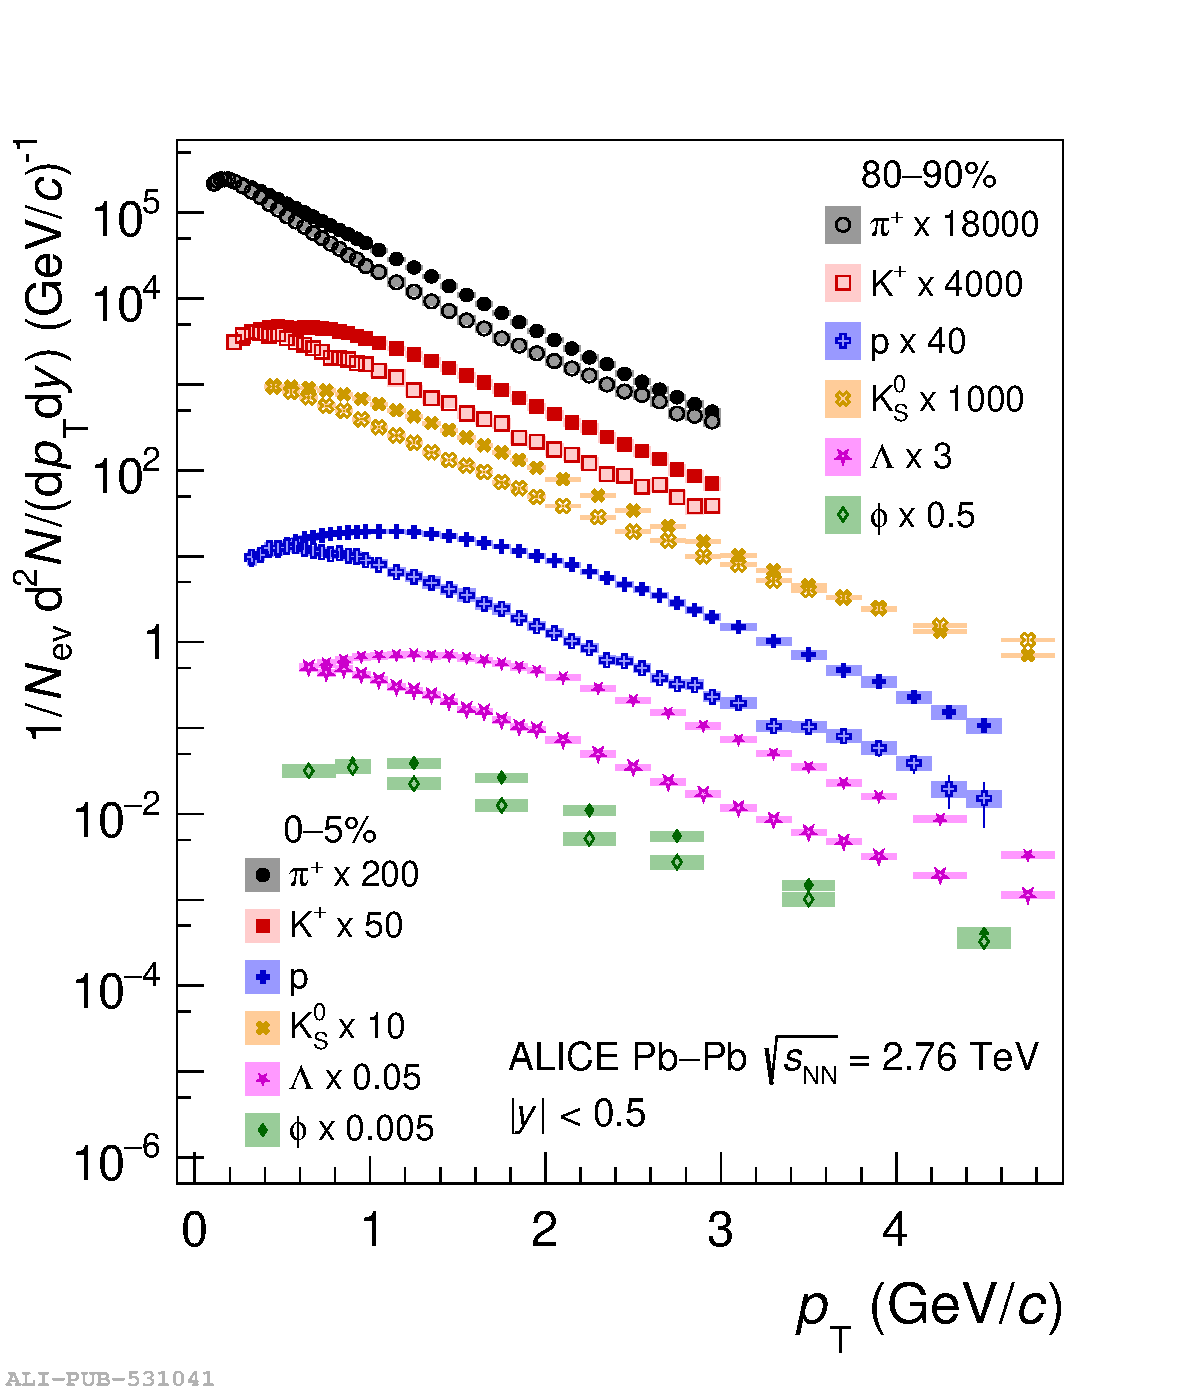
\includegraphics[width=0.7\linewidth]{Figures/Chapter 1/spectra_run1.pdf}
  \caption{Transverse momentum distributions of $\mathrm{\pi^+}$, $\mathrm{K^+}$, p, $\mathrm{K^0_s}$, $\mathrm{\Lambda}$, and $\mathrm{\phi}$ mesons for the 0--5\% and 80--90\% centrality intervals in Pb--Pb collisions at $\snn=2.76$ TeV measured by the ALICE experiment. The data points are scaled by various factors for better visibility. Taken from~\cite{ALICE:2022wpn}.}
  \label{fig:RadialFlow}
\end{figure}
After the chemical freeze-out, inelastic interactions between the hadrons do not take place anymore. However, elastic interactions can still occur, leading to a modification of the momentum distribution of the particles. By studying the transverse momentum spectra of the particles produced in the collision, it is possible to extract information on the produced system.

For a stationary thermal source with a temperature $T$, the Lorentz-invariant momentum distribution of the particles is given by:
\begin{equation*}
    E\frac{\de N}{\de^3p} = \frac{\de N}{\pt\de\pt\de\varphi\de y} = \frac{g_\mathrm{i}V}{(2\pi)^3} E \frac{1}{e^{(E-\mu_\mathrm{i})/T}\pm1}\quad ,
\end{equation*}
where $E$ is the energy of the particle, $g_\mathrm{i}$ and $\mu_\mathrm{i}$ are the degeneracy factor and chemical potential of the particles of species i, respectively, $V$ is the volume of the source, and the + sign is for fermions while the $-$ sign is for bosons. By using the relation
\begin{equation*}
  \frac{\de N}{\pt\de\pt} = \frac{\de N}{\mt\de\mt}\quad ,
\end{equation*}
and by assuming that $e^{(E-\mu_\mathrm{i})/T}\gg1$, the transverse momentum spectrum of particles can be obtained by integrating over the azimuthal angle $\varphi$ and the rapidity $y$, leading to:
\begin{equation}\label{eq:mt_scaling}
    \frac{\de N}{\mt\de\mt} = \frac{g_\mathrm{i}V}{(2\pi)^2} \mt e^{\mu_\mathrm{i}/T} K_1\left(\frac{\mt}{T}\right) \xrightarrow[\mt\gg T]{} V'\sqrt{\mt}e^{-\mt/T}\quad .
\end{equation}
From Eq.~\ref{eq:mt_scaling} emerges that for a stationary thermal particle source with a temperature $T$, the transverse mass spectrum of the particles follows an exponential distribution with a slope parameter $T$, and is independent of the particle species. This is known as the \mt-scaling of the transverse mass spectra, and is observed in pp and small-system collisions at low \sqs, with a slope parameter of $T\sim167$~MeV. However, in heavy-ion collisions, this description is not valid, as the QGP, which is a thermalised system of deconfined quarks and gluons, has a thermal pressure. The pressure difference between the QGP and the surrounding vacuum leads to a collective expansion of the fireball, which is called \emph{radial flow}. This causes the particles to be pushed in the transverse direction, causing a modification of the transverse momentum spectra of the particles, which is characterised by a shift of the spectra towards higher \pt values, with a more pronounced effect for heavier particles, as shown in Fig.~\ref{fig:RadialFlow}. The radial flow can also be defined as a correlation between the velocity of an element of the system and its space-time position, which is superimposed on the random thermal motion of the particles.

\begin{figure}[htb]
  \centering
  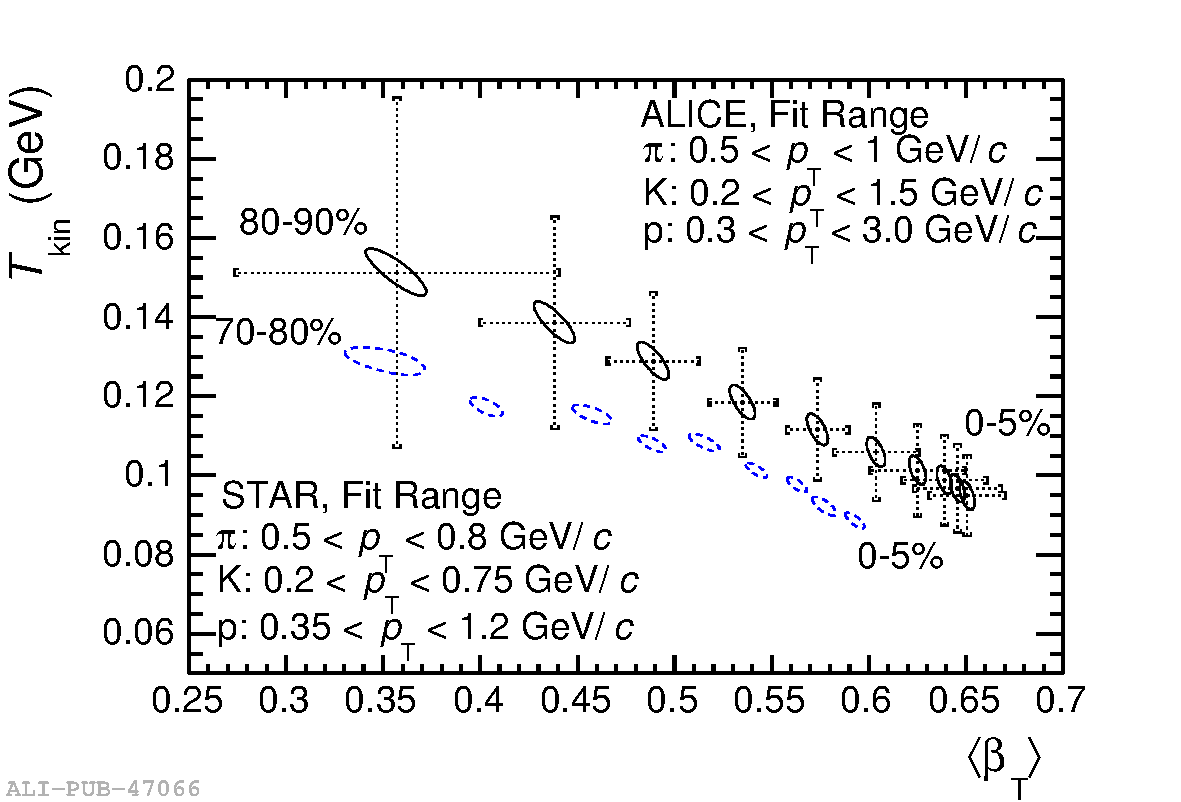
\includegraphics[width=0.7\linewidth]{Figures/Chapter 1/2014-Feb-27-cBlastWaveVsSTAR.pdf}
  \caption{Results of blast-wave fits obtained with the ALICE experiment at the LHC, compared to similar fits at RHIC energies, for different centrality intervals. Taken from~\cite{ALICE:2013mez}}
  \label{fig:blast_wave_fit}
\end{figure}

The radial flow can be described by using phenomenological models, such as the blast-wave model~\cite{Schnedermann:1993ws}, which assumes that the particles are emitted from a thermal source with a collective velocity field. It relies on the Cooper-Frye prescription~\cite{Cooper:1974mv}, which assumes an instantaneous freeze-out of the particles in the radial direction, to calculate the transverse momentum spectra of the particles in terms of the temperature of the source, the collective velocity field, and the transverse flow profile. Results from SPS, RHIC, and LHC experiments show that the transverse momentum spectra of the particles produced in heavy-ion collisions can be well described by the blast-wave model, with a temperature of the source of around 110--120 MeV, almost independent of \snn, and a collective velocity field of around 0.5--0.6~$c$ in the most central collisions, with a growing trend with \snn, as shown in Fig.~\ref{fig:blast_wave_fit}. Although the blast-wave model provides a good description of the transverse momentum spectra of the particles produced in heavy-ion collisions, it is important to note that the parameters wich are evaluated with this model are extracted by fitting the \mt spectra of the particles, and could not be directly related to the properties of the QGP. Hence, it is important to study whether more sophisticated models, such as hydrodynamics, can provide a more detailed description of the space-time evolution of the system.

Hydrodynamics-based models rely on energy and momentum conservation laws, which need to be expressed in a relativistic form due to the relativistic nature of the system:
\begin{equation*}
    \partial_\mu T^{\mu\nu} = 0\quad ,~\mathrm{with}\quad T^{\mu\nu} = (\varepsilon + p)u^\mu u^\nu - p g^{\mu\nu}\quad ,
\end{equation*}
where $T^{\mu\nu}$ is the energy-momentum tensor, $\varepsilon$ is the energy density, $p$ is the pressure, $u^\mu$ is the four-velocity of the fluid element, and $g^{\mu\nu}$ is the metric tensor. An additional condition comes from the conservation of the baryon number, which is expressed as:
\begin{equation*}
    \partial_\mu (n_B u^\mu) = 0\quad ,
\end{equation*}
where $n_B$ is the baryon density. A further equation is needed to close the system of equations, and is provided by the equation of state of the QGP, which relates the pressure to the energy density and the baryon density. As the fireball is in a non-equilibrium state in the early stages of the collision, the hydrodynamics equations need an initial condition to describe the system. This is usually provided by the Glauber model~\cite{Miller:2007ri}, which describes the collision of the two nuclei as a superposition of nucleon-nucleon collisions, and provides the initial energy density profile of the system. Monte Carlo simulations describing partonic showers such as UrQMD~\cite{Bleicher:1999xi} and AMPT~\cite{Lin:2004en} can also be used to provide the initial conditions for the hydrodynamics models. \\
The hydrodynamics calculations provide a good description of the transverse momentum spectra of the particles produced in heavy-ion collisions, and the emerging parameters are similar to those obtained with the blast-wave model. In addition, hydrodynamics calculations and their extensions, such as viscous hydrodynamics, can be used to study other observables, such as the elliptic flow, which is a measure of the anisotropy of the particle emission in the transverse plane.

\subsection{High-$\mathbf{\pt}$ hadrons and jet quenching}\label{sec:high_pt}
\begin{figure}[htb]
  \centering
  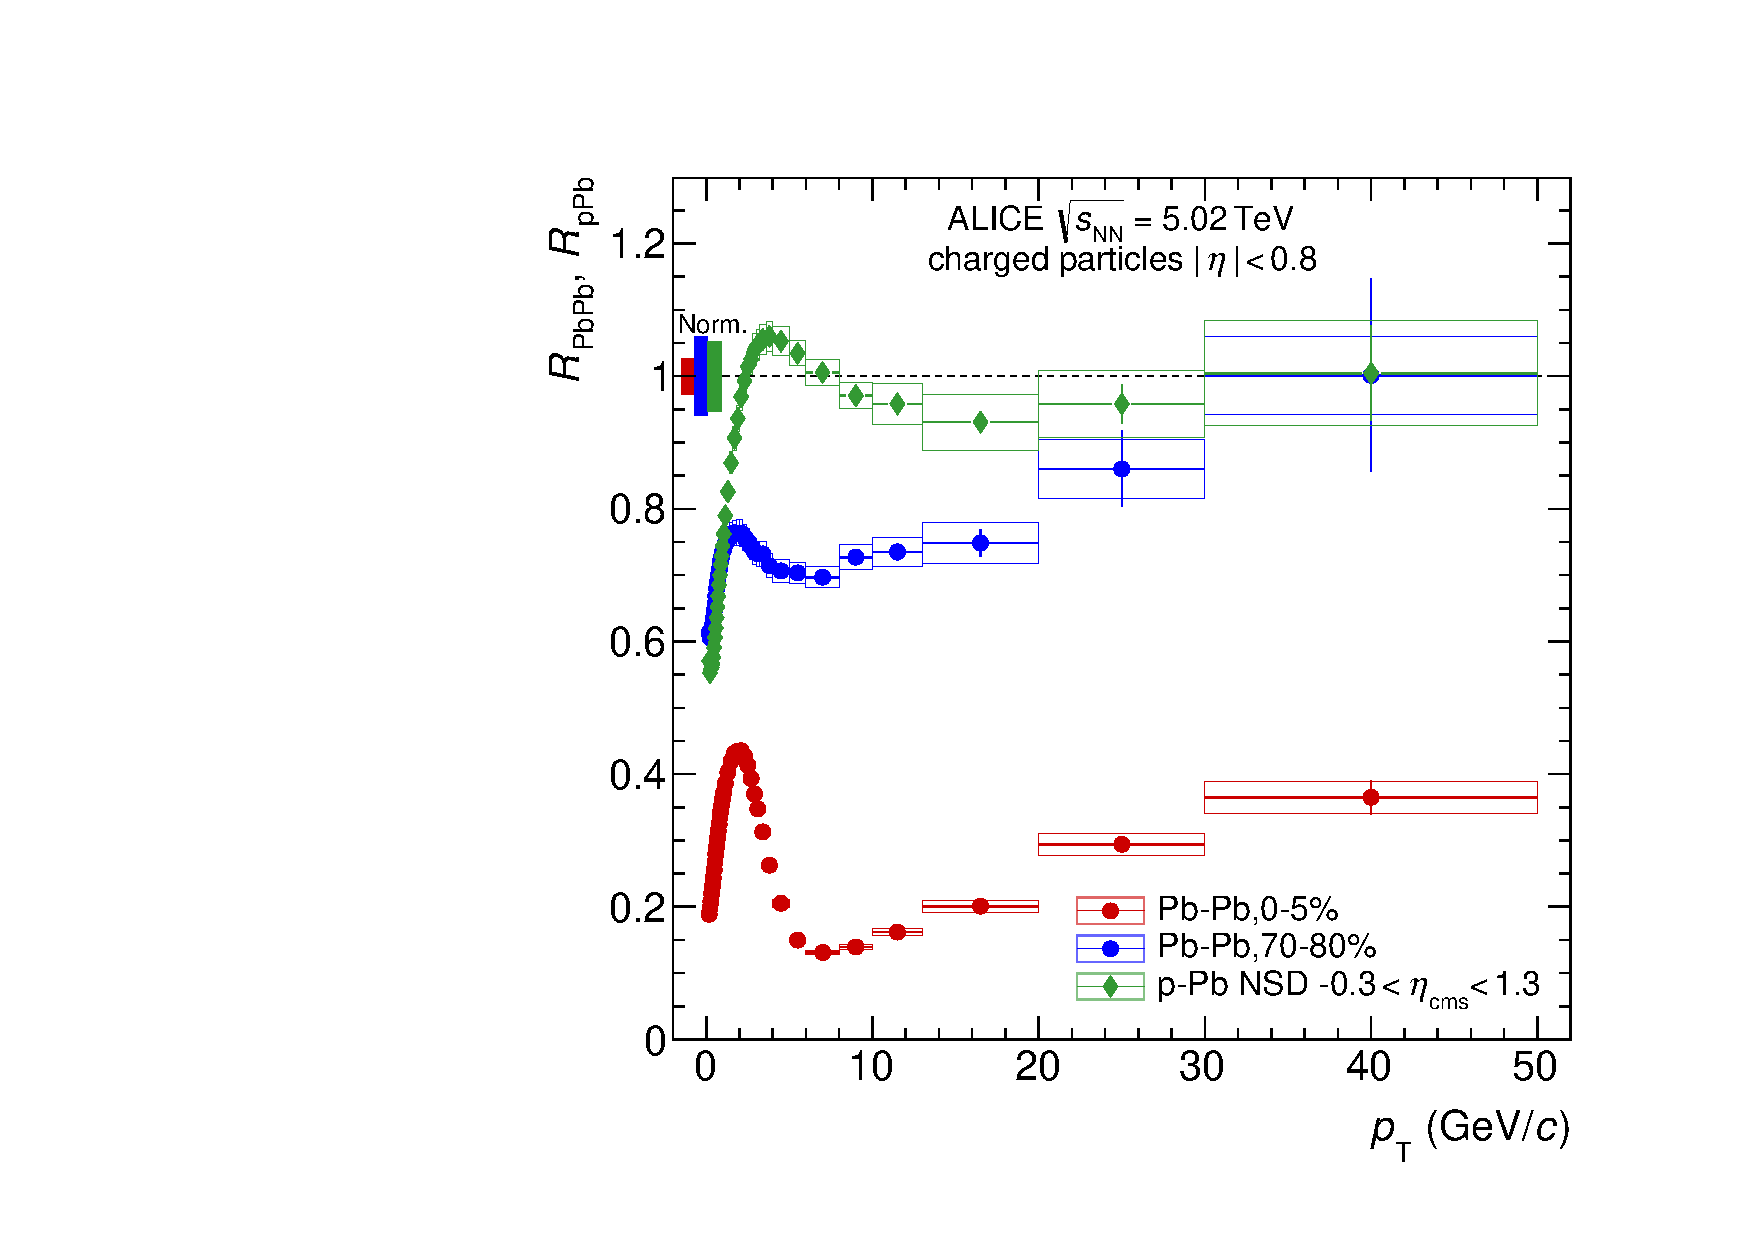
\includegraphics[width=0.7\linewidth]{Figures/Chapter 1/rAArpPb.pdf}
  \caption{Nuclear modification factors measured by ALICE in central $(0-5\%)$ and peripheral $(70-80\%)$ Pb--Pb collisions at $\snn=13$~TeV and in p--Pb collisions at $\snn = 13$~TeV. Taken from~\cite{ALICE:2018vuu}.}
  \label{fig:RAA}
\end{figure}

High-\pt partons are produced in hard-scattering processes, i.e. those with a high momentum transfer. As such, they are typically produced in the early stages of the collision and experience the whole fireball evolution. They can be therefore used to probe the properties of the earliest stages of the QGP. The Glauber model predicts the production cross-section of hard-scattering processes to scale with the number of binary nucleon-nucleon collisions. To test this prediction, the nuclear modification factor, $R_\mathrm{AA}$, is defined as the ratio of the \pt-differential hadron yield in heavy-ion collisions to the one in proton-proton collisions, scaled by the mean number of binary nucleon-nucleon collisions $\langle N_\mathrm{coll} \rangle$ :
\begin{equation*}
    R_\mathrm{AA} = \frac{\de N_\mathrm{AA}/\de\pt}{\langle N_\mathrm{coll} \rangle~\de N_\mathrm{pp}/\de\pt}\quad .
\end{equation*}
As the \pt increases, the production mechanism becomes harder, and it is expected that the nuclear modification factor approaches unity, namely \emph{binary scaling}. However, experimental results~\cite{ALICE:2018vuu} show that the nuclear modification factor is suppressed at high \pt, with a suppression that increases with the centrality of the collision. This is due to both initial-state effects, such as the Cronin effect~\cite{Kopeliovich:2002yh}, which can be studied in proton-nucleus collisions where the production of QGP is not expected, and to final-state effects, due to the presence of the QGP. Partons traversing the QGP lose energy through elastic scatterings with the partons of the medium, and via gluon radiation, which is the dominant process for high-energy partons. The energy loss can be estimated in the BDMPS formalism~\cite{Baier:1996kr}, which assumes that the radiated gluon gets de-coherent from the emitting parton through multiple soft scatterings with the medium constituents. The energy loss of the partons is quantified as:
\begin{equation*}
    \Delta E = \frac{1}{4}\alpha_s C_\mathrm{R}\hat{q}L^2\quad ,
\end{equation*}
Where \als is the strong coupling constant, $C_\mathrm{R}$ is the Casimir factor, which is 3 for gluon-gluon couplings and 4/3 for quark-gluon interactions, $\hat{q}$ is the transport coefficient, and $L$ is the path length of the parton in the medium. The transport coefficient is related to the energy-density of the medium, as $\hat{q} \propto \varepsilon^{3/4}$, so that energy loss measurements can be used to infer the properties of the QGP. Typical energy losses of high-\pt partons traversing the whole QGP are of the order of 40 GeV, which is a significant fraction of the parton energy. The energy loss of the partons leads to a suppression of the high-\pt hadron spectra, which consequently leads to a suppression of the nuclear modification factor at high \pt. 

\begin{figure}[htb]
  \centering
  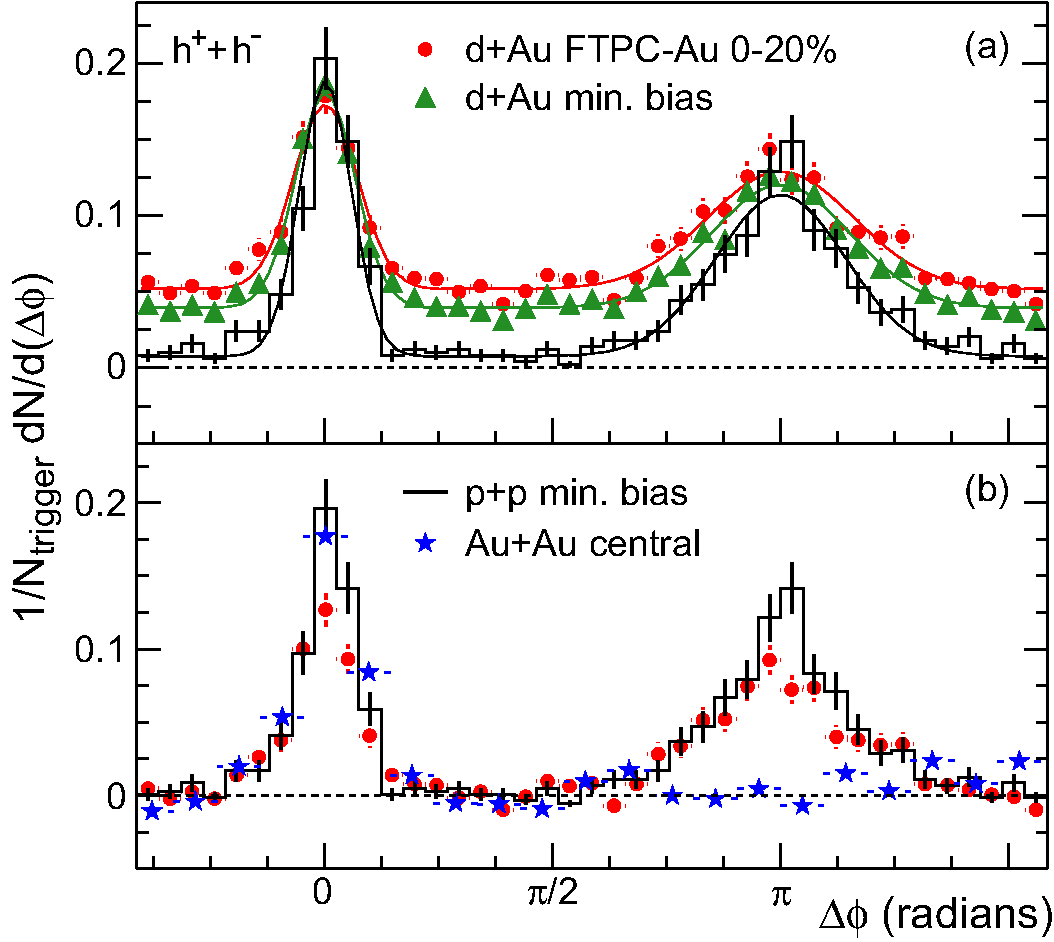
\includegraphics[width=0.7\linewidth]{Figures/Chapter 1/dAu_Fig4.pdf}
  \caption{Top: Two-particle azimuthal distributions for minimum bias and central d--Au collisions, and for proton-proton collisions at $\snn = 200$~GeV measured by the STAR Collaboration. Bottom: Comparison of pedestals-subtracted two-particle azimuthal distributions for central d--Au collisions to those seen in proton-proton and central Au--Au collisions. Taken from~\cite{STAR:2003pjh}.}
  \label{fig:azimuthal_correlations}
\end{figure}

At leading order, partons are produced in back-to-back pairs, forming what is known as di-jets. The parton shower generated by the jet pointing in the direction of the medium is expected to lose more energy than the one pointing in the opposite direction, leading to what is known as \emph{jet quenching}. These interactions can be studied by measuring two-particle azimuthal distribution correlations of the produced hadrons. For each event, the particle with the highest \pt above a certain threshold is selected, and the azimuthal angle of other high-\pt particles is measured with respect to the first one. For proton-proton and proton-nucleus collisions, the azimuthal distribution presents two peaks: the \emph{near-side peak}, which is found at $\phi=0$ and is due to the hadrons produced in the same jet as the trigger particle, and the \emph{away-side peak}, which is found at $\phi=\pi$ and is due to the hadrons produced in the opposite jet. In heavy-ion collisions, the away-side peak is suppressed due to the energy loss in the QGP, as shown in Fig.~\ref{fig:azimuthal_correlations}.

In addition, the QGP can also affect the hadronisation process. In small colliding systems, such as pp and p--Pb collisions, hadronisation occurs via fragmentation, where the colour string holding together a quark-antiquark pair breaks, producing another quark-antiquark pair. This process leads to the production of a collimated jet of hadrons with \pt lower than the one of the first quark-antiquark pair. When the QGP is produced, another hadronisation mechanism becomes available, as the QGP is a thermalised system: the coalescence (or recombination) mechanism. Low \pt partons close in the velocity-space phase space can bind together to form a higher-\pt hadron. This enhances the production of baryons, as the \pt-distribution of partons inside the QGP follows a rapidly decreasing trend.

\subsection{Strangenness enhancement}
One of the first proposed signatures of the QGP formation is the strangeness enhancement~\cite{Rafelski:1982pu}, which refers to the observation of an increased production of strange hadrons in heavy-ion collisions compared to proton-proton collisions. At a microscopic level, the enhancement of strange hadrons is a direct consequence of the high energy densities reached in the collisions, which allow for the thermal production of strange quarks and antiquarks. Strange quarks are not present as valence quarks in the initial state, and can be produced in hard $2\rightarrow 2$ scatterings ($gg\rightarrow s\overline{s}, q\overline{q}\rightarrow s\overline{s}$), or via gluon splitting ($g\rightarrow s\overline{s}$) during the evolution of the system. While these processes are dominant for the production of strange hadrons with high \pt, at low \pt the production of strange hadrons is dominated by non-perturbative processes. At a macroscopic level, the enhancement of the production of strange hadrons can be explained using a statistical approach, in a framework known as the statistical hadronisation model. In this model, the system is described as an ideal gas of hadrons and resonances, which is assumed to be in thermal and chemical equilibrium at the chemical freeze-out. The hadrons production in heavy-ion collisions is described according to a grand-canonical ensemble statistical distribution, which depends on the temperature and the chemical potentials of the system. In a grand-canonical ensemble, which is used to describe a system that exchanges both energy and particles with a reservoir, the energy and quantum numbers are only conserved on average on a large volume. The description of the hadrons production in smaller colliding systems, such as $\mathrm{e^+e^-}$ and pp collisions, requires the use of a canonical ensemble, which is used to describe a system that exchanges only energy with a reservoir, and requires the exact (local) conservation of the quantum numbers. This leads to a suppression of strange quark production as compared to the grand canonical ensemble. 

The strangeness enhancement in heavy-ion collisions has been observed in several experiments, such as the STAR experiment at RHIC~\cite{STAR:2007cqw} and the ALICE experiment at the LHC~\cite{ALICE:2013xmt}. In addition, an enhancement of strange hadrons has been observed in small systems, such as pp~\cite{ALICE:2016fzo} and p-Pb~\cite{ALICE:2013wgn, ALICE:2015mpp} collisions, in high-multiplicity events, and follows a hierarchy determined by the hadron strangeness. This observation is intriguing, as QGP production is not expected in such systems. Furthermore, several effects such as azimuthal correlations and mass-dependent hardening of \pt distributions, which are typically associated with QGP formation in nuclear collisions, have been observed in these systems. Could small droplets of QGP be formed in these collisions? Could other mechanisms explain the observed effects? These are still open questions in the field of high-energy nuclear physics, and they are the subjects of ongoing research.

Figure~\ref{fig:StrangenessEnhancement} shows the \pt-integrated yield ratios of strange (\kzs, $\Lambda$) and multi-strange ($\Xi^\pm, \Omega^\pm$) hadrons to pions ($\pi^++\pi^-$) as a function of the charged particle multiplicity density, $\braket{\de N_\mathrm{ch}/\de\eta}$, measured in $\lvert y\rvert<0.5$ in different collision systems (pp, p--Pb and Pb--Pb) using the ALICE experiment at the LHC~\cite{ALICE:2016fzo}. The data show a clear enhancement of strange to non-strange hadron production with increasing multiplicity. At the highest multiplicities, the yield ratios saturate at values that are compatible with what is measured in central Pb-Pb collisions, where QGP is formed.

\begin{figure}[htb!]
  \centering
  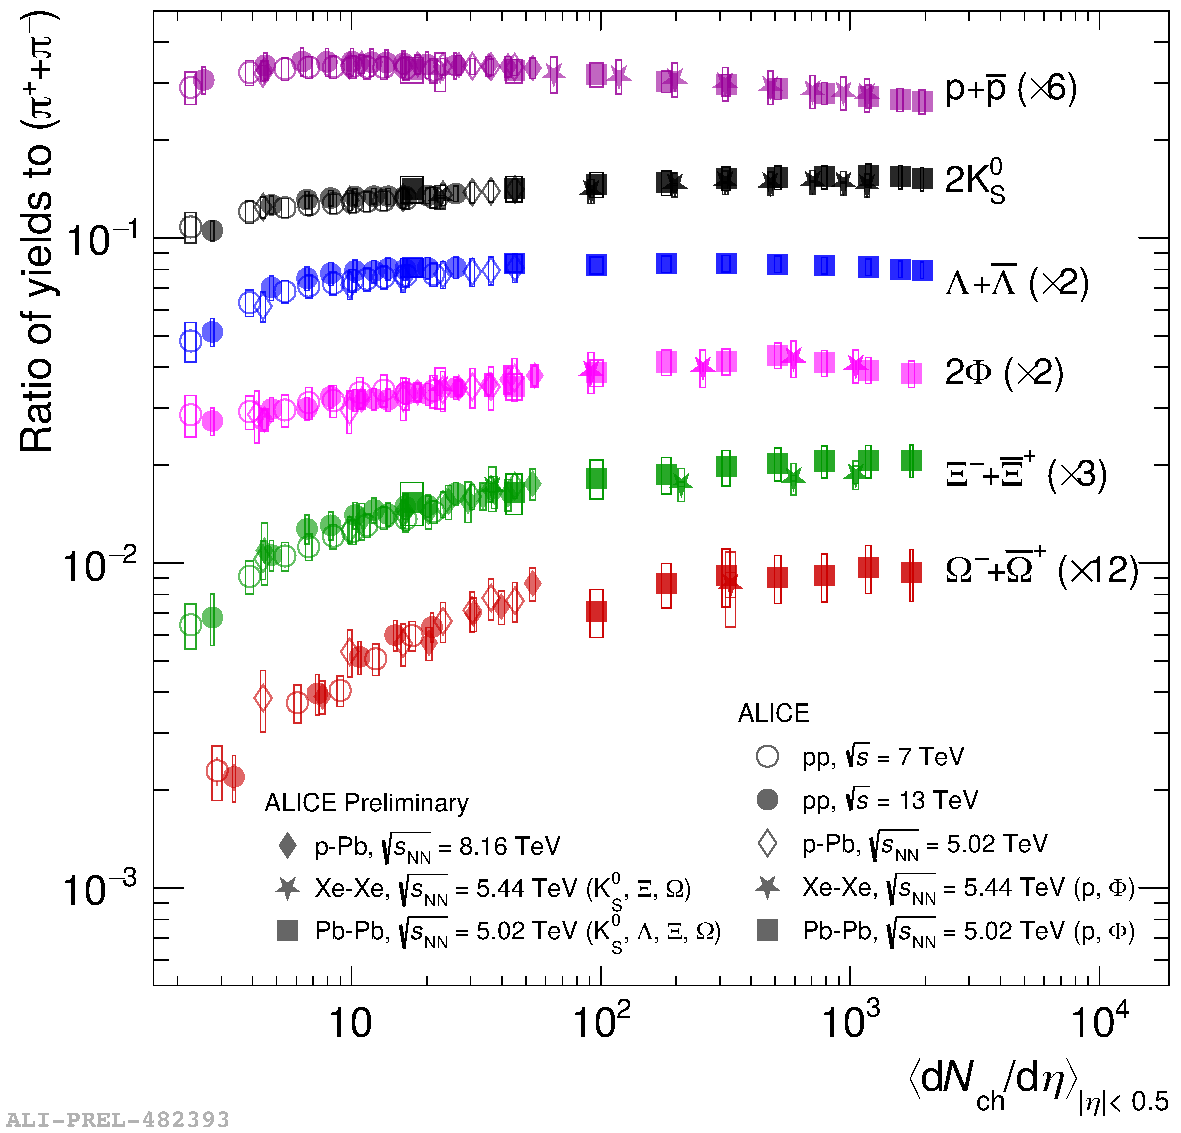
\includegraphics[width=0.7\linewidth]{Figures/Chapter 1/img_ToPionRatios_1.pdf}
  \caption{\pt--integrated yield ratios of strange (\kzs, $\Lambda$) and multi-strange ($\Xi^\pm, \Omega^\pm$) hadrons to pions ($\pi^++\pi^-$) as a function of $\braket{\de N_\mathrm{ch}/\de\eta}$ measured in pp, p--Pb and Pb--Pb collisions at midrapidity$(\lvert y\rvert<0.5)$. Taken from~\cite{ALICE_figures}.}
  \label{fig:StrangenessEnhancement}
\end{figure}


%In the QGP, strange quarks are produced through the interactions between the quarks and gluons, and they can form strange hadrons, such as the $\Lambda$, $\Xi$, and $\Omega$ baryons. The production of strange hadrons in heavy-ion collisions is a key signature of the QGP, and it has been observed in several experiments, such as the ALICE experiment at the LHC~\cite{ALICE:2022wpn}. The strangeness enhancement is a direct consequence of the high energy densities reached in the collisions, which allow for the production of strange quarks and antiquarks. In the QGP, strange quarks are produced through the interactions between the quarks and gluons, and they can form strange hadrons, such as the $\Lambda$, $\Xi$, and $\Omega$ baryons. The production of strange hadrons in heavy-ion collisions is a key signature of the QGP, and it has been observed in several experiments, such as the ALICE experiment at the LHC~\cite{ALICE:2022wpn}.